\usetikzlibrary{calc}


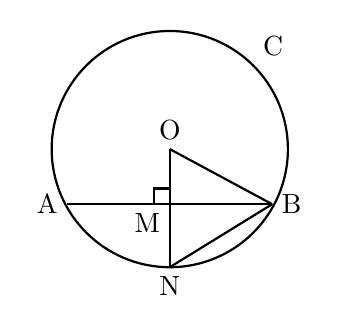
\begin{tikzpicture}[scale=1]

    % Define the center of the circle
    \coordinate (O) at (0,0);

    % Draw the circle
    \draw[thick] (O) circle (1.5);

    % Define coordinates for the points on the circle and chord
    % AB is the horizontal chord
    \coordinate (A) at (-1.3, -0.7);
    \coordinate (B) at (1.3, -0.7);
    
    % M is the midpoint of AB, where the perpendicular line intersects
    \coordinate (M) at (0, -0.7);
    
    % C is a point on the top right of the circle
    \coordinate (C) at (45:1.5);

    % N is the point at the bottom of the circle where the perpendicular line meets
    \coordinate (N) at (0, -1.5);

    % Draw the chord AB
    \draw[thick] (A) -- (B);

    % Draw the line connecting O, M, and N
    \draw[thick] (O) -- (N);

    % Draw the line from O to B
    \draw[thick] (O) -- (B);

    % Draw the line from N to B
    \draw[thick] (N) -- (B);

    % Draw the right-angle symbol at M
    \draw[thick] (M) ++(-0.2,0) -- ++(0,0.2) -- ++(0.2,0);

    % Add labels for the points
    \node[left] at (A) {A};
    \node[right] at (B) {B};
    \node[above right] at (C) {C};
    \node[above] at (O) {O};
    \node[below left] at (M) {M};
    \node[below] at (N) {N};

\end{tikzpicture}